\section{Integrales de línea: campos escalares y vectoriales}

\begin{definición}[Camino]
Un camino (o curva paramétrica) en $\mathbb{R}^n$ es una función continua $\gamma: I \to \R^n$ donde $I \subset \R$ es un intervalo. \\
Si $\gamma$ es diferenciable en un punto $t \in I$, entonces el vector velocidad de $\gamma$ en el punto (instante) $t$ es el vector tangente a la curva en ese punto, es decir, el vector:
$$\gamma'(t) = (\gamma_1'(t), \ldots, \gamma_n'(t)) \text{ si } \gamma = (\gamma_1, \ldots, \gamma_n)$$
\end{definición}

\begin{definición}[Longitud de un camino]
Sea $\gamma: [a,b] \to \R^n$ un camino en $\R^n$. Sea $\sigma = \{a = t_1 < t_2 < \ldots < t_n = b\}$ partición de $[a,b]$. Definimos $$\Sigma(\gamma, \sigma) = \sum_{i = 1}^{n} \lVert \gamma(t_i) - \gamma(t_{i-1}) \rVert $$
Definimos entones la longitud de $\gamma$ como: $$L(\gamma) = \sup\{\Sigma(\gamma, \sigma) \ | \  \sigma \text{ es una partición de } [a, b]\} \in [0, + \infty]$$
Decimos que $\gamma$ es \textbf{rectificable} si $L(\gamma) < + \infty$.
\end{definición}

\begin{observación}
Existen caminos continuos que no son rectificables. Por ejemplo, la curva de Peano, el copo de nieve de Koch o la dada por:
$$l(\gamma) \geq \sum_{n = 1}^{N}\frac{1}{n} \forall n \in \mathbb{N} \text{ luego } l(\gamma) \geq \sum_{n = 1}^{\infty}\frac{1}{n} = + \infty$$
\end{observación}

\begin{definición}[Camino $C^1$ a trozos]
Decimos que un camino $\gamma: [a, b] \to \mathbb{R}^n$ es $C^1$ a trozos si:
$$\exists \mathcal{P} = \{a = t_0 < t_1 < \ldots < t_n = b\}$$ tal que $\gamma|_{[t_{i-1}, t_i]}$ es $C^1$ para todo $i = 1, \ldots, n$.
\end{definición}

\begin{observación}
En cada intervalo $[t_{i-1}, t_i]$ la función $\gamma$ es $C^1$, es decir, en los extremos admite derivadas laterales, aunque puede ocurrir que sean distintas.
\end{observación}

\begin{teorema}
    Sea $\gamma: [a, b] \to \mathbb{R}^n$ un camino $C^1$ a trozos. Entonces $\gamma$ es rectificable y su longitud es:
    $$l(\gamma) = \int_{a}^{b} \lVert \gamma'(t) \rVert dt$$
\end{teorema}

\begin{observación}
Tenemos que $t \to  \lVert \gamma'(t) \rVert $ existe, y es continua, salvo quiza en un número finito de puntos, luego en particular es integrable en sentido Riemann y en sentio Lebesgue.
\\Además, si $\mathcal{P} = \{t_0 = a < t_1 < \ldots < t_n = b\}$ es partición de $[a,b]$ entonces:
\[
    \int_{a}^{b}  \lVert \gamma'(t) \rVert dt = \sum_{i = 1}^{n} \int_{t_{i-1}}^{t_i} \lVert \gamma'(t) \rVert dt
\]
\end{observación}

Para la demostración del teorema anterior, veamos un lema previo:
\begin{lema}
    Sea $\gamma: [a, b] \to \mathbb{R}^n$ camino continuo entonces se cumple que:
    $$ \lVert \int_{a}^{b} \gamma(t)dt \rVert  \leq \int_{a}^{b} \lVert \gamma(t) \rVert dt$$
    donde:
    $$\int_{a}^{b} \gamma(t)dt = \left(\int_{a}^{b} \gamma_1(t)dt, \ldots, \int_{a}^{b} \gamma_n(t)dt \right)\in \mathbb{R}^n$$
\end{lema}
\begin{proof}
    Hagamos una distinción de casos:
    \begin{itemize}
        \item Si $u = \int_a^b \gamma(t)dt = 0$
        \item Si $u = \int_a^b \gamma(t)dt \neq 0$, sea $u \in \mathbb{R}^n$ con $ \lVert u
                  \rVert = 1 \implies$ $$ \lVert v \rVert = \langle u, v \rangle = \sum_{i =
                      1}^{u} u_i \int_{a}^{b} \gamma_i(t)dt = \int_{a}^{b} \sum_{i = 1}^{n} u_i
                  \gamma_i(t)dt \leq \int_{a}^{b} \lVert \gamma(t) \rVert dt = \lVert
                  \int_{a}^{b} \gamma(t)dt \rVert $$
    \end{itemize}
\end{proof}

\begin{proof}
    Veamos ahora la demostración del teorema: \\
    Podemos suponer que $\gamma: [a, b] \to \mathbb{R}^n$ es $C^1$ en casi todo $[a, b]$.
    \begin{enumerate}
        \item Veamos que $l(\gamma) \leq \int_{a}^{b} \lVert \gamma'(t) \rVert dt$: \\ Sea
              $\mathcal{P} = \{a = t_0 < t_1 < \ldots < t_n = b\}$ partición de $[a, b]$.
              Entonces: $$\Sigma(\gamma, \mathcal{P}) = \sum_{i = 1}^{n} \lVert \gamma(t_i) -
                  \gamma(t_{i-1}) \rVert = \sum_{i = 1}^{n} \lVert
                  \int_{t_{i-1}}^{t_i}\gamma'(t)dt \rVert \leq \sum_{ i =
                      1}^{n}\int_{y_{i-1}}^{t_i} \lVert \gamma'(t) \rVert dt = \int_{a}^{b} \lVert
                  \gamma'(t) \rVert dt \quad \forall \text{ partición } \mathcal{P}$$ Luego,
              tomando el supremo de todas las particiones, obtenemos que $l(\gamma) \leq
                  \int_{a}^{b} \lVert \gamma'(t) \rVert dt$
        \item Como $t \to \lVert \gamma'(t) \rVert $ es continua en casi todo $[a,
                          b]$-compacto, luego es uniformemente continua en $[a, b]$.\\ Dado $\epsilon >
                  0, \exists \delta > 0$ tal que si $t,s \in [a, b]$ y $|t-s| < \delta \implies
                  \lVert \gamma'(t) - \gamma'(s) \rVert < \epsilon$\\ Sea $\mathcal{P} = \{a =
                  t_0 < t_1 < \ldots < t_n = b\}$ partición de $[a, b]$ con $t_i - t_{i-1} <
                  \delta \quad \forall i = 1, \ldots, n$\ $$\int_{t_{i-1}}^{t_i} \lVert
                  \gamma'(t) \rVert dt \leq \int_{t_{i-1}}^{t_i} \lVert \gamma'(t_i) \rVert +
                  \epsilon dt = \lVert \gamma(t_i) \rVert \cdot (t_i - t_{i -1}) + \epsilon(t_1 -
                  t_{i-1})$$ $$= \lVert \int_{t_{i-1}}^{t_i}\gamma'(t)dt \rVert + \epsilon(t_i -
                  t_{i-1}) = \lVert (\gamma_1'(t_i), \ldots, \gamma_n'(t_i)) \rVert \cdot (t_i -
                  t_{i-1}) + \epsilon(t_i - t_{i-1})$$ $$ \leq \int_{t_{i -1}}^{t_i}(\gamma'(t_i)
                  - \gamma'(t)dt)dt +\int_{t_{i-1}}^{t_i} \lVert \gamma'(t) \rVert dt +
                  \epsilon(t_i - t_{i-1})$$ $$ \leq \int_{t_{i-1}}^{t_i} \lVert \gamma'(t_i) -
                  \gamma'(t) \rVert dt + \int_{t_{i-1}}^{t_i} \lVert \gamma'(t) \rVert dt +
                  \epsilon(t_i - t_{i-1}) \leq 2\epsilon(t_i - t_{i-1}) + \int_{t_{i-1}}^{t_i}
                  \lVert \gamma'(t) \rVert dt$$ $$ = 2\epsilon(t_i - t_{i-1})\cdot \lVert
                  \gamma(t_i) - \gamma(t_{i-1}) \rVert $$ Luego, $$\int_{a}^{b} \lVert \gamma'(t)
                  \rVert dt = \sum_{i = 1}^n \int_{t_{i-1}}^{t_i} \lVert \gamma'(t) \rVert dt
                  \leq \sum_{i = 1}^{n}2\epsilon(t_i - t_{i-1}) + \lVert \gamma(t_i) -
                  \gamma(t_{i-1}) \rVert = 2\epsilon(b-a) + \Sigma(\gamma, \mathcal{P}) \leq
                  2\epsilon(b-a) + l(\gamma)$$ Todo esto está sacado del libro de Facenda,
              Fremiche.
    \end{enumerate}
\end{proof}

\ejemplo{
    Sea la curva parametrizada
    \[
        \gamma: [0, 2\pi] \to \mathbb{R}^2, \quad \gamma(t) = (\cos t, \sin t).
    \]

    Además, se cumple que
    \[
        \gamma(0) = (1,0) = p.
    \]
    Derivando, obtenemos
    \[
        \gamma'(t) = (-\sin t, \cos t),
    \]
    y en particular,
    \[
        \gamma'(0) = (0,1) = \vec{v}.
    \]

    \subsection*{Cambio de parámetro}

    Consideremos el cambio de variable $t = 2\pi s$ con $0 \leq s \leq 1$.
    Definiendo la nueva curva
    \[
        \sigma(s) = (\cos(2\pi s), \sin(2\pi s)), \quad 0 \leq s \leq 1,
    \]
    obtenemos su derivada:
    \[
        \sigma'(s) = (2\pi (-\sin(2\pi s)), 2\pi \cos(2\pi s)).
    \]
    En particular, en $s = 0$,
    \[
        \sigma'(0) = 2\pi (0,1) = (0,2\pi).
    \]

    \subsection*{Otro cambio de parámetro}

    Si realizamos el cambio $t = -2\pi s$, obtenemos la curva
    \[
        \alpha(s) = (\cos(2\pi s), -\sin(2\pi s)).
    \]
    Calculamos su derivada:
    \[
        \alpha'(s) = (2\pi (-\sin(2\pi s)), -2\pi \cos(2\pi s)).
    \]
}

\begin{definición}
Sea $\gamma : [a,b] \to \mathbb{R}^n$ camino $C^1$ a trozos y sea $f:Im\gamma \to \mathbb{R}$ continua \\
Diremos que $f$ es un campo escalar sobre $Im\gamma$ \\
Definimos:
$$ \int_{\gamma} f = \int_{a}^{b} f(\gamma(t)) \cdot  \lVert \gamma'(t) \rVert dt$$ \\

Notacion: Podemos denotar $$\int_{\gamma} f = \int_{\gamma} f ds$$ \\ Ademas
$$\l(\gamma) = \int_{a}^{b} \lVert \gamma'(t) \rVert dt = \int_{a}^{b} ds$$
\end{definición}

\begin{definición}
Dos caminos $\gamma: [a,b] \to \mathbb{R}^n$ y $\sigma:[c,d] \to \mathbb{R^n}$ son equivalentes si: \\
$$ \exists h:[c,d] \to [a,b] $$ homeomorfismo $C^1$ que cumple ademas que \\
$$h' \neq 0$$ en $[c,d]$ tal que ademas $$[a,b] \to_{\gamma} \mathbb{R}^n \leftarrow_\sigma [c,d] \leftrightarrow_{h} [a,b]$$ \\
Tenemos ademas que: $\sigma = \gamma \circ h$ con $\sigma(s) = \gamma(h(s))$ $\forall s \in [c,d]$ \\
Ahora, por el teorema de Bolzano tenemos dos posibilidades:
\begin{enumerate}
    \item Si $h'>0$ es decir, $h$ es creciente, decimos que h conserva la orientacion (o
          que $\gamma$ y $\sigma$ tienen la misma orientacion)
    \item Si $h'<0$ es decir, $h$ es decreciente, decimos que $h$ invierte la orientacion
          ($\gamma$ y $\sigma$ tienen orientacion opuesta)
\end{enumerate}
\end{definición}

\begin{observación}
\vspace{-2.5em}
\begin{enumerate}
    \item Si $h:[c,d] \to [a,b]$ es biyectiva y $C^1$ con $h' \neq 0$ entonces aplicando
          el Teorema de la funcion inversa obtenemos que $h$ admite inversa local al
          rededor de cada punto. \\ Ademas se cumple que $(h^{-1})'(h(s)) =
              \frac{1}{h'(s)}$ $\forall s \in [c,d]$ \\ Como ademas $h$ es biyectiva la
          inversa local coincide con la inversa global, luego $h:[c,d] \to [a,b]$ es un
          difeomorfismo $C^1$, es decir, $\exists h^{-1}:[a,b] \to [c,d]$ que es $C^1$
    \item Usando esto obtenemos que la equivalencia de caminos es una relacion de
          equivalencia.
\end{enumerate}
\end{observación}

\begin{observación}
Si $K\subset \mathbb{R}^n$ compacto y $h:K \to H\subset \mathbb{R^n}$ es continua y biyectiva, entonces $h:K \to H$ es un homeomorfismo.
\end{observación}

\begin{proof}
    Tenemos que $h:K \to H$ es biyectiva, luego $\exists h^{-1}:H \to K$, veamos que es biyectiva. \\
    Dado $C \subset K$ cerrado $\implies$ $C$ es compacto $\implies$ $h(C)$ es compacto $\implies$ $(h^{-1})^{-1}(C)=h(C)$ que es compacto en $H$, luego es cerrado en $H$ \\
\end{proof}

\begin{teorema}
    Sean $\gamma: [a,b] \to \mathbb{R}^n$ y $\gamma:[c,d] \to \mathbb{R}^n$ caminos $C^1$ a trozos equivalentes. \\
    Sea ademas $f:Im(\gamma)=Im(\sigma) \to \mathbb{R}$ continua, entonces: \\
    $$\int_{\gamma}f=\int_{\sigma}f$$
\end{teorema}

\begin{observación}
Si $\gamma$ y $\sigma$ son equivalentes $\implies Im(\gamma)=Im(\sigma)$
\end{observación}

\begin{proof}
    Tenemos $h:[c,d] \to [a,b]$ difeomorfismo $C^1$ con $\gamma \circ h = \sigma$ con ademas $\sigma(s) = \gamma(h(s)) \implies \sigma'(s) = \gamma'(h(s))h'(s)=h'(s)\gamma'(h(s))$ \\
    \begin{enumerate}
        \item Caso 1: $h$ es creciente $(h'>0)$ \\ $$\int_{\gamma} f = \int_{t=a}^{t=b}
                  f(\gamma(t)) \lVert \gamma'(t) \rVert dt = \int_{s=c}^{s=d} f(\gamma(h(s)))
                  \lVert \gamma'(h(s)) \rVert h'(s)ds$$ \\ Haciendo ahora el cambio $t=h(s)$ y
              $dt=h'(s)ds$ obtenemos: $$\int_{s=c}^{s=d} f(\sigma(h(s))) \lVert \sigma'(s)
                  \rVert ds=\int_{\sigma}f$$
        \item Caso 2: $h$ es decreciente $(h'<0)$\\ Tenemos $$ \int_{\gamma} f=
                  \int_{t=a}^{t=b} f(\gamma(t)) \lVert (\gamma'(t)) \rVert
                  dt=\int_{s=d}^{s=c}f(\gamma(h(s))) \lVert \gamma'(h(s)) \rVert h'(s)ds$$ \\
              Haciendo ahora el cambio $t=h(s)$ y $dt=h'(s)ds$ obtenemos: $$\int_{s=c}^{s=d}
                  f(\gamma(h(s))) \lVert \gamma'(h(s)) \rVert (-h'(s))ds = \int_{\sigma}f$$
    \end{enumerate}
\end{proof}

\begin{corolario}
    Si $\gamma$ y $\sigma$ son equivalentes y $C^1$ a trozos $\implies l(\gamma)=l(\sigma)$
\end{corolario}

\begin{proof}
    $$l(\gamma) =\int_{\gamma}1=\int_{a}^{b} \lVert \gamma'(t) \rVert dt=\int_{\sigma}1=l(\sigma)$$
\end{proof}

\begin{definición}
Sea $\gamma:[a,b] \to \mathbb{R^n}$ camino $C^1$ a trozos. Definimos el camino inverso como: \\
$$(-\gamma):[a,b] \to \mathbb{R^n}$$ como $$ (-\gamma)(s)=\gamma(a+b-s)$$
\end{definición}

\begin{observación}
De hecho, $(-\gamma)$ es equivalente a $\gamma$ con $(-\gamma)(s)=\gamma(h(s))$ luego $Im(-\gamma)=Im(\gamma)$
\end{observación}

\begin{definición}[Concatenacion de caminos]
Sean $\gamma:[a,b] \to \mathbb{R^n}$ y $\sigma:[c,d] \to \mathbb{R^n}$ caminos $C^1$ a trozos con $\gamma(b)=\sigma(c)$\\
Definimos su concatenacion como:\\
$$\gamma + \sigma:[a,b+(d-c)] \to \mathbb{R^n}$$
$$(\gamma + \sigma) = \begin{cases}
        \gamma(t), \text{ si } a \leq t \leq b \\
        \sigma(t - b + c) \text{ si } b\leq t \leq b+(d-c)
    \end{cases}$$
\end{definición}

\begin{observación}
En este caso, si
\[
    f : \operatorname{Im}(\gamma_1) \cup \dots \cup \operatorname{Im}(\gamma_m) \longrightarrow \mathbb{R}
\]
es continua en las curvas, entonces se cumple:
\[
    \int_{\gamma_1 + \dots + \gamma_m} f = \sum_{i=1}^{m} \int_{\gamma_i} f
\]
\end{observación}

\ejemplo{

Dado el camino \(\gamma\) definido por:
\[
    \gamma : [0, 2\pi] \to \mathbb{R}^3 \qquad \gamma(t) = (\underbrace{\cos(t)}_{x(t)}, \, \underbrace{\sin(t)}_{y(t)}, \, \underbrace{t}_{z(t)})
\]

Y la funcion \(f : \mathbb{R}^3 \to \mathbb{R}\) dada por:

\[
    f(x,y,z) = x^2 + y^2 + z^2
\]

Entonces, calcular la integral de \(f\) a lo largo de \(\gamma\).

\[
    x^2(t) + y^2(t) = 1 \qquad  \gamma(0) = (1, 0, 0), \quad \gamma(2\pi) = (1, 0, 2\pi)
\]

\[
    \gamma'(t) = (-\sin(t), \, \cos(t), \, 1), \quad \|\gamma'(t)\| = \sqrt{\sin^2(t) + \cos^2(t) + 1} = \sqrt{2}
\]

\[
    \int_{\gamma} f = \int_0^{2\pi} \left( \cos^2(t) + \sin^2(t) + t^2 \right) \sqrt{2} \, dt = \int_0^{2\pi} (1 + t^2) \sqrt{2} \, dt = \left[ t + \frac{t^3}{3} \right]_0^{2\pi} \sqrt{2} = \left( 2\pi + \frac{8\pi^3}{3} \right) \sqrt{2}
\]

}

\subsection{Campos Vectoriales}

\begin{definición} [Campo Vectorial]
Sea $A \subset \mathbb{R}^n$, un campo vectorial continuo en $A$ es una función continua $\vec{F} : A \to \mathbb{R}^n$ que asigna a cada punto $x \in A$ un vector $\vec{F}(x) \in \mathbb{R}^n$.
\end{definición}
\begin{definición} [Integral de un Campo Vectorial a lo largo de un Camino]
Sea $\gamma : [a, b] \to \mathbb{R}^n$ un camino $\mathcal{C}^1$ a trozos y $\vec{F} : \operatorname{Im}(\gamma) \to \mathbb{R}^n$ un campo vectorial continuo. Se define la integral de $\vec{F}$ a lo largo de $\gamma$ como:
\[
    \int_\gamma \vec{F} = \int_a^b \langle \vec{F}(\gamma(t)), \gamma'(t) \rangle dt
\]
\end{definición}

\begin{observación}
El producto escalar $\langle \vec{F}(\gamma(t)), \gamma'(t) \rangle$ representa la proyección ortogonal del vector $\vec{F}(\gamma(t))$ en la dirección de la tangente a $\gamma \text{ en } \gamma(t)$.
\definecolor{ccqqqq}{rgb}{0.8,0,0}
\definecolor{ududff}{rgb}{0.30196078431372547,0.30196078431372547,1}
\definecolor{qqwuqq}{rgb}{0,0.39215686274509803,0}

\begin{center}
    \begin{tikzpicture}[line cap=round,line join=round,>=triangle 45,x=1cm,y=1cm]
        \begin{axis}[
                x=1cm,y=1cm,
                axis lines=middle,
                xmin=-2,
                xmax=3.5,
                ymin=-0.6805806893374612,
                ymax=3.6,
                xtick={-2.5,-2,...,4.5},
                ytick={-0.5,0,...,4.5},
                xticklabels=\empty, % Remove x-axis labels
                yticklabels=\empty % Remove y-axis labels
            ]
            \clip(-2.9040233036492373,-0.6805806893374612) rectangle (4.931567305660256,4.6842052156427245);
            \draw[line width=0.75pt,color=qqwuqq,smooth,samples=100,domain=-2.9040233036492373:4.931567305660256] plot(\x,{sin(((\x))*180/pi)+1.5});
            \draw[line width=0.75pt,color=ccqqqq,smooth,samples=100,domain=-2.9040233036492373:4.931567305660256] plot(\x,{sqrt(3)/2*(\x)+1/2-(3.141592653589793*sqrt(3))/12+1.5});
            \draw [->,line width=0.75pt] (0.5,2) -- (-0.15030877559829892,2.71444);
            \begin{scriptsize}
                \draw[color=qqwuqq] (0.7,1.7) node {$\gamma(t)$};
                \draw [fill=ududff] (0.5,2) circle (1pt);
                \draw[color=ccqqqq] (2.5,3) node {$\gamma'(t)$};
                \draw[color=black] (-0.7, 2.291892925953723) node {$\vec{F}(\gamma(t))$};
            \end{scriptsize}
        \end{axis}
    \end{tikzpicture}
\end{center}

\end{observación}

\textbf{Notación:}\\
Si
\[
    \gamma(t) = (x_1(t), \ldots, x_n(t)) \quad \text{y} \quad \gamma'(t) = (x_1'(t), \ldots, x_n'(t))
\]
entonces:
\[
    \int_\gamma \vec{F} = \int_a^b \langle \vec{F}(x_1(t), \ldots, x_n(t)), (x_1'(t), \ldots, x_n'(t)) \rangle dt
\]
\[
    = \int_a^b \left[ F_1(\gamma(t)) x_1'(t) + \cdots + F_n(\gamma(t)) x_n'(t) \right] dt = \int_\gamma F_1 \, dx_1 + \cdots + F_n \, dx_n
\]
donde $dx_i = x_i'(t) dt$, para $i = 1, \ldots, n$ y $\vec{F} = (F_1, \ldots,
    F_n)$.

\begin{teorema}
    Sean $\gamma : [a, b] \to \mathbb{R}^n$ y $\sigma : [c, d] \to \mathbb{R}^n$ caminos $\mathcal{C}^1$ a trozos y equivalentes, y sea $\vec{F} : \operatorname{Im}(\gamma) = \operatorname{Im}(\sigma) \to \mathbb{R}^n$ un campo vectorial continuo. Entonces:
    \vspace{-0.5em}
    \begin{enumerate}
        \item $\displaystyle \int_\gamma \vec{F} = \int_\sigma \vec{F}$ \quad si $\gamma$ y $\sigma$ tienen la misma orientación.
        \item $\displaystyle \int_\gamma \vec{F} = - \int_\sigma \vec{F}$ \quad si $\gamma$ y $\sigma$ tienen orientación opuesta.
    \end{enumerate}
\end{teorema}

\begin{proof}
    Sabemos que existe $h: [c,d] \to [a,b]$, biyección de clase $C^1$ con $h' \neq 0$, tal que:

    \[
        \begin{tikzcd}
            {[a,b]} \arrow[r, "\gamma"] & \operatorname{Im}(\sigma) \\
            {[c,d]} \arrow[u, "h"] \arrow[ur, "\sigma"']
        \end{tikzcd}
    \]
    Luego
    \[ \sigma'(s) = \gamma'(h(s)) h'(s), \quad \forall s \in [c,d]. \]

    Distinguimos dos casos según la orientación de los caminos:

    \begin{itemize}
        \item \textbf{Caso 1: Misma orientación}\\
              Si $r$ y $\sigma$ tienen la misma orientación, entonces $h' > 0$ (es decir, $h$ es creciente). Se tiene que:
              \[
                  \int_{\gamma} \vec{F} = \int_{t=a}^{t=b} \langle \vec{F} (\gamma (t)), \gamma'(t) \rangle dt = \int_{s=c}^{s=d} \langle \vec{F} (\gamma(h(s))), \gamma'(h(s)) \rangle h'(s) ds
              \]
              \[
                  = \int_{s=c}^{s=d} \langle \vec{F} (\sigma(s)), \sigma'(s) \rangle ds = \int_{\sigma} \vec{F}
              \]
              Donde el cambio de variable viende dado por:
              \[
                  \begin{cases}
                      t = h(s) \\
                      dt = h'(s) ds
                  \end{cases}
              \]
        \item \textbf{Caso 2: Orientación opuesta}\\
              Si $\gamma$ y $\sigma$ tienen orientación opuesta, entonces $h' < 0$ (es decir, $h$ es decreciente). En este caso:
              \[
                  \int_{\gamma} \vec{F} = \int_{t=a}^{t=b} \langle \vec{F} (\gamma(t)), \gamma'(t) \rangle dt = \int_{s=d}^{s=c} \langle \vec{F} (\gamma(h(s))), \gamma'(h(s)) \rangle h'(s) ds
              \]
              \[
                  = -\int_{s=c}^{s=d} \langle \vec{F} (\sigma(s)), \sigma'(s) \rangle ds = -\int_{\sigma} \vec{F}
              \]
    \end{itemize}
\end{proof}

\begin{observación}
Dado una camino continuo $\gamma : [a, b] \to \mathbb{R}^n$ cualesquiera y un campo vectorial continuo $\vec{F} : \operatorname{Im}(\gamma) \to \mathbb{R}^n$, se cumple que:
\vspace{-0.5em}
\begin{enumerate}
    \item $\int_{-\gamma} \vec{F} = -\int_{\gamma} \vec{F}$.
    \item $\int_{\gamma_1+\ldots+\gamma_2} \vec{F} = \sum_{i=1}^{n} \int_{\gamma_i} \vec{F}$.
\end{enumerate}
\end{observación}

\ejemplo{
Un camino puede ser diferenciable (ó $C^1$) y, sin embargo, su imagen puede presentar "picos". Por ejemplo, el camino $\gamma : [-1, 1] \to \mathbb{R}^2$ dado por $\gamma(t) = (t^3, |t^3|)$ es $C^1$ en el intervalo $[-1, 1]$, pero su imagen presenta un pico en el origen. En efecto,

\[
    \gamma'(t) = (\gamma_1'(t), \gamma_2'(t)) \quad \text{con} \quad \gamma_1'(t) = 3t^2 \quad \text{y} \quad \gamma_2'(t) = \begin{cases} 3t^2 & \text{si } t \geq 0 \\ -3t^2 & \text{si } t < 0 \end{cases}
\]

\[
    \gamma_2'(0) = \lim_{t \to 0} \frac{\gamma_2(t) - \gamma_2(0)}{t} = \lim_{t \to 0} \frac{t^2|t|-0}{t} = \lim_{t \to 0} t|t| = 0
\]

Luego $\gamma'(0)$ existe y además $\gamma'(0) = (0, 0)$. Sin embargo, la
imagen de $\gamma$ en el origen presenta un pico, lo que implica que la curva
no es regular en ese punto.

}

\begin{definición} [Camino Simple y Regular]
Diremos que una función \( \gamma: [a,b] \to \mathbb{R}^n \) es un \textbf{camino simple y regular} si:
\vspace{-0.5em}
\begin{itemize}
    \item \( \gamma \) es continua.
    \item \( \gamma \) es inyectiva (simple).
    \item \( \gamma \) es de clase \( C^1 \) en \( [a,b] \) y cumple que \( \gamma'(t) \neq 0 \) para todo \( t \in [a,b] \).
\end{itemize}
\end{definición}

\begin{observación}
\begin{enumerate}
    \vspace{-2.5em}
    \item En este caso, la función \( \gamma: [a,b] \to \operatorname{Im}(\gamma) \) es
          un homeomorfismo sobre su imagen.
    \item Diremos que \( C \subset \mathbb{R}^n \) es una \textbf{curva simple y regular}
          si \( C = \operatorname{Im}(\gamma) \), donde \( \gamma \) es un camino simple
          y regular. En este caso, \( \gamma \) es una \textbf{parametrización simple y
              regular} de \( C \).
\end{enumerate}
\end{observación}

\ejemplo{
    Consideremos la curva:
    \[
        C = \{(x,y) \in \mathbb{R}^2 \mid x^2 + y^2 = 1, \quad y > 0 \}.
    \]

    \begin{center}
        \begin{tikzpicture}
            % Axes
            \draw[->] (-1.5, 0) -- (1.5, 0) node[right]{$x$}; % x-axis
            \draw[->] (0, -0.5) -- (0, 1.5) node[above]{$y$}; % y-axis

            % Upper semicircle (centered at origin)
            \draw (1, 0) arc[start angle=0, end angle=180, radius=1];
            \node at (0, 1) [above right]{$1$};

            % Label
            \node at (1.2, 1.2) {$C$};
        \end{tikzpicture}
    \end{center}

    Una posible parametrización es:
    \[
        \gamma: [0, \pi] \to \mathbb{R}^2  \qquad \gamma(t) = (\cos (t) \sin (t))
    \]
    Su derivada es:
    \[
        \gamma'(t) = (-\sin (t), \cos (t)) \neq (0,0), \quad \forall t \in (0,\pi).
    \]
    Por lo tanto, \( \operatorname{Im}(\gamma) = C \), confirmando que \( \gamma \)
    es una parametrización simple y regular de \( C \). }

\begin{teorema}
    Sea \( C \subset \mathbb{R}^n \) una curva simple y regular y sean \( \gamma \) y \( \sigma \) parametrizaciones simples y regulares de \( C \). Entonces, \( \gamma \) y \( \sigma \) son equivalentes.
\end{teorema}

\ejemplo{
    Un segimento en $\mathbb{R}^n$: DAdos $p \neq q$ en $\mathbb{R}^n$, el segmento $[p,q]$ se define como:
    $$[p,q] = \{(1 - t)p + t1  0 \leq t \leq 1\} = C \text{ es una curva simple regular}$$
    $$C = Im(\gamma) \text{ donde } \gamma:[0,1] \to [p,q] \text{con } \gamma(t) = (1-t)p + tq = q +t(p-q)$$
    Tenemos que $\gamma$ es biyectiva y $\gamma'(t) = p-q \neq 0$ $\forall t \in [0,1]$
}
\ejemplo{
Una gráfica en $\mathbb{R}^n$: Sea $g: [a, b] \to \mathbb{R}$ de clase $C^1$. La gráfica $G_g = \{(t, g(t) : a \leq t \leq b)\}$ es una curva simple regualr en $\mathbb{R}^2$ con $G_g = Im(\gamma)$ donde $\gamma:[a,b] \to G_g$ es de clase $C^1$ y biyectiva con $\gamma(t) = (t, g(t))$ y $\gamma'(t) = (1, g'(t)) \neq \vec{0}$ $\forall t \in [a,b]$
}

\begin{observación}
Si $\gamma: [a,b] \to \mathbb{R}^n$ es una curva simple regular, entones $\gamma$ es un homeomorfismo sobre su imagen, i.e. $\gamma: [a, b] \to C = Im(\gamma)$ es un homeomorfismo. \\
Falta demostrar que $\gamma^{-1}: C \to [a,b]$ es continua.\\
Si no fuera así: Sea $x_0 \in C$ tal que $\gamma^{-1}$ no es continua en $x_0$ entonces $\exists \epsilon > 0$ tal que $\forall \delta = \frac{1}{k} > 0, \exists x_k \in C$ con $ ||x_k - x_0|| \leq \frac{1}{k}$ pero $||\gamma^{-1}(x_k) - \gamma^{-1}(x_0)|| > \epsilon$ \\
$\forall k \in \N$, denotemos $(t_k)_{k \in \N} = (\gamma^{-1}(x_k)) \subset [a,b]$-compacto $\implies \exists (t_{k_j}) \to t_0 \in [a,b]$ y como $\gamma$ es continua $\implies \gamma(t_{k_j}) \to \gamma(t_0) \equiv (x_{k_j}) \to x_0$ \\
Luego $x_0 = \gamma(t_0) \iff t_0 = \gamma^{-1}(x_0)$. Pero $t_{k_j} = \gamma^{-1}(x_{k_j})$ satisface que $||t_{k_j} - t_0|| \geq \epsilon \iff ||\gamma^{-1}(x_{k_j}) - \gamma^{-1}(x_0)|| \geq \epsilon$ lo cual es una contradicción.
\end{observación}

\begin{proof}
    A continuación viene la demostración del teorema anterior: \\
    Sean $\sigma: [c,d] \to Im(\sigma)$ y $\gamma: [a,b] \to Im(\gamma)$ tales que $Im(\sigma) = C = Im(\gamma)$.
    Dado que $\sigma$ y $\gamma$ son homeomorfismos sobre $C$ entonces $\exists h: [c,d] \to [a,b]$ homeomorfismo $C^1$ tal que $h = \gamma^{-1} \circ \sigma$.
    Entonces falta demostrar que $h$ es de clase $C^1$ con $h' \neq 0$ en $[c,d]$
    Sea $s_0 \subset [c,d]$ y denotaremos $x_0 = \sigma(s_0)$
    \begin{itemize}
        \item     Consideramos primero el caso de que $s_0 \in (c,d)$ y sea $t_0 \in (a, b)$ tal
              que $\gamma(t_0) = x_0$: Sabemos que $gamma'(t_0) = (\gamma_1'(t_0), \ldots,
                  \gamma_n'(t_0)) \neq \vec{0}$ Supongamos que $\gamma_1'(t_0) \neq 0$ entonces
              definamos la función $H: (a, b) \times \mathbb{R}^{n-1} \to \mathbb{R}^{n}
                  \implies H(t, y_2, \ldots, y_n) = (\gamma_1(t), \gamma_2(t) + y_2, \ldots,
                  \gamma_n(t) + y_n) \text{ y } H(t_0, 0, \ldots, 0) = (\gamma_1(t), \ldots,
                  \gamma_n(t)) = \gamma(t)$ \\ $$DH(t, 0 \ldots 0) = \begin{pmatrix}
                      \gamma_1'(t) & 0      & \ldots & 0      \\
                      \gamma_2'(t) & 1      & \ldots & 0      \\
                      \vdots       & \vdots & \ddots & \vdots \\
                      \gamma_n'(t) & 0      & \ldots & 1
                  \end{pmatrix} \implies det(DH(t, 0 \ldots 0)) = \gamma_1'(t) \neq 0$$
              Entonces por el Teorema de la Función Inversa $\exists U^{(t_0, 0, \ldots 0)} \subset (a, b)$ y $\exists V^{x_0}$ tal que $H: U^{(t_0, 0, \ldots 0)} \to V^{x_0}$ es un difeomorfismo de clase $C^1$. Definimos $F: V^{x_0} \to \mathbb{R}$ tal que $F(x) = \pi_1(H^{-1}(x)) \in (a,b)$ donde $\pi_1$ es la proyección en la primera coordenada. \\
              $$F(\gamma(t)) = \pi_1(H^{-1}(\gamma(t))) = \pi_1(H^{-1} \circ H(t, 0, \ldots, 0)) = \pi_1(t, 0, \ldots, 0) = t$$
              Si $t = h(s)$ entonces $F(\gamma(h(s))) = F(\sigma(s))$ luego $h$ es de clase $C^1$ alrededeor de $s_0$. Además, $\sigma'(s_0) = (\gamma \circ h)'(s_0) = \gamma(t_0) \circ h'(s_0) \implies h'(s_0) \neq 0$ \\
        \item Para los exteriores de $c$ y $d$ se usa que: $\sigma: [c,d] \to \mathbb{R}^n$
              es de clase $C^1$ entonces $\exists \bar{\sigma}: (c - \epsilon, d + \epsilon)
                  \to \mathbb{R}^n$ extensión de clase $C^1$ y además $\bar{\sigma}' \neq 0$ en
              $(c - \epsilon, d + \epsilon)$
    \end{itemize}
\end{proof}
\begin{definición}
Sea $C \subset \mathbb{R}^n$ curva simple regular entonces;
\begin{enumerate}
    \item Si $f: C \to \mathbb{R}$ es continua, se define $\int_{C} f = \int_{\gamma} f$
          siendo $\gamma$ una parametrización simple y regular de $C$
    \item Una orientación de $C$ se define como un sentido de recorrido de $C$, es decir,
          señalar un origen y un extremo de $C$. Si $C$ está orientada y $\vec{F}: C \to
              \mathbb{R}^n$ es un campo vectorial continuo, se define $\int_{\vec{C}} \vec{F}
              = \int_{\gamma} \vec{F}$ siendo $\gamma$ una parametrización simple y regular
          de $C$, que conserva la orientación o que induce en $C$ la orientación elegida. \end{enumerate}
\end{definición}

\begin{observación}
Si cambiamos de orientación: $\int_{C^-} \vec{F} = -\int_{C} \vec{F}$
\end{observación}

\begin{definición}
Diremos que $C \subset \R^n $ es una curva regular simple a trozos si $C = Im(\gamma)$ siendo $\gamma$ camino $C^1$ a trozos con $\gamma = \gamma_1 + \ldots + \gamma_k$ y cada $\gamma_j$ es simple y regular $\forall j = 1, \ldots, k$\\
En este caso si $C_j = Im(\gamma_j) \forall j = 1, \ldots, k$ entonces denotaremos $C = C_1 + \ldots + C_k$ y definimos para $f: C \to \R$ continua: $\int_{C} f = \sum_{j=1}^{k} \int_{C_j} f$
\end{definición}

\begin{observación}
Se puede demostrar que el resultado no depende de la partición de $C$ en curvas simples y regulares (descomposición).
\end{observación}

\begin{observación}
Si $C = C_1 + \ldots + C_k$ tienen orientaciones coherentes (el extremo de $C_j$ coincide con $C_{j+1} \forall j = 1, \ldots, k-1$) diremos que $C$ está orientada y definimos para un campo vectorial $\vec{F}: C \to \R^n$ continua: $\int_{C} \vec{F} = \sum_{j=1}^{k} \int_{C_j} \vec{F}$
\end{observación}

\subsection{Campos Conservativos}

\begin{definición}
Sea un conjunto $U  \subset \mathbb{R}^n$ abierto. Un campo vectorial-$C^1$ continuo $\vec{F}: U \to \mathbb{R}^n$ se dice que es conservativo (ó campo gradiente) si $\exists \varphi: U \to \mathbb{R}$ de clase $C^1$ tal que $\vec{F} = \nabla \varphi \iff \vec{F} = (F_1, \ldots, F_n)$ donde $F_i = \frac{\partial \varphi}{\partial x_i} \quad \forall i = 1, \ldots, n$.
Se dice entonces que la función $\varphi$ es un potencial de $\vec{F}$.
\end{definición}

\begin{observación}
Si $\varphi$ es un potencial de $\vec{F}$ entonces también lo es de $\vec{F} + a \quad \forall a \in \mathbb{R}^n$ constante.
\end{observación}

\begin{proposición}
Sean $U \subset \mathbb{R}^n$ abierto y $\vec{F}: U \to \mathbb{R}^n$ un campo conservativo y $\gamma: [a,b] \to U$ un camino $C^1$ a trozos. Entonces:
$$\int_{\gamma} \vec{F} = \varphi(\gamma(b)) - \varphi(\gamma(a))$$
donde $\varphi$ es un potencial de $\vec{F}$.
\end{proposición}

\begin{proof}
    Distinguimos dos casos:
    \begin{enumerate}
        \item \textbf{Caso 1:} $\gamma$ es $C^1$ en $[a,b]$\\
              Definimos la función $g: [a,b] \to \mathbb{R}$ de forma que $g(t) = \varphi(\gamma(t))$ y aplicamos la regla de la cadena:
              \[
                  \begin{tikzcd}
                      {[a,b]} \arrow[d, "\gamma"'] \arrow[r, "g"] & \mathbb{R} \\
                      U \arrow[ru, "\varphi"']
                  \end{tikzcd}
              \]
              En particular tenemos que $g$ es de clase $C^1$ y además:
              \[
                  g'(t) = (\varphi \circ \gamma)'(t) = D\varphi (\gamma(t)) (\gamma'(t)) = \langle \nabla \varphi (\gamma(t)), \gamma'(t) \rangle = \langle \vec{F}(\gamma(t)), \gamma'(t) \rangle
              \]

              \[
                  \int_{\gamma} \vec{F} = \int_{a}^{b} \langle \vec{F} (\gamma(t)), \gamma'(t) \rangle dt = \int_{a}^{b} g'(t) dt \overset{\text{TFC}}{=} g(b) - g(a) = \varphi (\gamma(b)) - \varphi (\gamma(a))
              \]

        \item \textbf{Caso 2:} \(\gamma\) es \(C^1\) a trozos

              Se aplica el caso 1 a cada trozo.
    \end{enumerate}
\end{proof}

\begin{teorema} [Caracterización de los Campos Conservativos]
    Sea el conjunto $U \subset \mathbb{R}^n$ abierto y conexo, y $\vec{F}: U \to \mathbb{R}^n$ un campo vectorial continuo, entonces son equivalentes:
    \begin{enumerate}
        \item El campo $\vec{F}$ es conservativo.
        \item $\int_{\gamma} \vec{F} = 0$ para todo $\gamma$ camino cerrado $C^1$ a trozos en $U$.
        \item $\int_{\gamma} \vec{F}$ solamente depende de los extremos de $\gamma$ para todo $\gamma$ camino $C^1$ a trozos en $U$.
        \item $\int_{\sigma} \vec{F} = 0$ para todo $\sigma$ poligonal cerrado de lados paralelos a los ejes coordenados en $U$.
        \item $\int_{\sigma} \vec{F}$ solamente depende de los extremos de $\sigma$ para todo $\sigma$ poligonal cerrado de lados paralelos a los ejes coordenados en $U$.
    \end{enumerate}

\end{teorema}

\begin{proof}
    \leavevmode
    \begin{itemize}
        \item $(1) \implies (2)$: Si $\gamma$ es un camino cerrado, entonces $\gamma(a) = \gamma(b)$ y por la proposición anterior:
              \[
                  \int_{\gamma} \vec{F} = \varphi(\gamma(b)) - \varphi(\gamma(a)) = \varphi(\gamma(b)) - \varphi(\gamma(b)) = 0
              \]
        \item $(2) \implies (3)$: Sean $\gamma_1$ y $\gamma_2$ caminos $C^1$ a trozos con los mismos extremos. Consideramos $\gamma = \gamma_1 + (-\gamma_2)$, que es un camino cerrado. Por hipótesis, $\int_{\gamma} \vec{F} = 0$, y por la proposición anterior:
              \[
                  0 = \int_{\gamma} \vec{F} = \int_{\gamma_1 + (-\gamma_2)} \vec{F} = \int_{\gamma_1} \vec{F} - \int_{\gamma_2} \vec{F} \implies \int_{\gamma_1} \vec{F} = \int_{\gamma_2} \vec{F}
              \]
        \item $(2) \implies (4)$ y $(3) \implies (5)$: trivial
        \item $(4) \implies (5):$ es análogo a $(2) \implies (3)$.
        \item $(5) \implies (1):$ Consideramos un punto \(x \in U\) y un vector unitario \(e_i\) en la dirección del eje \(i\)-ésimo. Tomamos un segmento de línea recta \(\gamma\) que va de \(x\) a \(x + h e_i\), donde \(h\) es un número real pequeño.

              La integral de \(\vec{F}\) sobre \(\gamma\) es:
              \[
                  \int_{\gamma} \vec{F} \cdot d\vec{r} = \varphi(x + h e_i) - \varphi(x)
              \]

              Dividiendo ambos lados por \(h\) y tomando el límite cuando \(h \to 0\),
              obtenemos:
              \[
                  \lim_{h \to 0} \frac{\varphi(x + h e_i) - \varphi(x)}{h} = \frac{\partial \varphi}{\partial x_i}(x)
              \]

              Por otro lado, la integral de \(\vec{F}\) sobre \(\gamma\) también se puede
              expresar como:
              \[
                  \int_{\gamma} \vec{F} \cdot d\vec{r} = \int_{0}^{h} \vec{F}(x + t e_i) \cdot e_i \, dt
              \]

              Tomando el límite cuando \(h \to 0\), obtenemos:
              \[
                  \lim_{h \to 0} \frac{1}{h} \int_{0}^{h} \vec{F}(x + t e_i) \cdot e_i \, dt = \vec{F}(x) \cdot e_i = F_i(x)
              \]

              Luego
              \[
                  \frac{\partial \varphi}{\partial x_i}(x) = F_i(x) \implies \nabla \varphi = \vec{F}
              \]
    \end{itemize}
\end{proof}

\begin{observación}
Un poligonal $\sigma$ de lados paralelos a los ejes es un camino $\sigma = \gamma_1 + \ldots + \gamma_k$ con $\gamma_j$ segmentos de recta paralelos a los ejes coordenados.\\
Además en este caso, si fijamos un punto $p \in U$ la función $\varphi: U \to \mathbb{R}$ definida por
\[
    \varphi(x) = \int_{\gamma_x} \vec{F} = \int_{p}^{x} \vec{F} \quad \text{donde } \gamma_x \text{ es un camino de } p \text{ a } x
\]
es un potencial de $\vec{F}$ en $U$.
\end{observación}

\begin{lema}
    Sea el conjunto $U \subset \mathbb{R}^n$ abierto y conexo. Dados los puntos $p, x \in U$, entonces existe $\sigma$ poligonal de lados paralelos a los ejes coordenados en $U$ tal que $\sigma$ une $p$ con $x$.
\end{lema}

\begin{proof}
    Sea el conjunto $$A = \{x \in U \mid \text{existe } \sigma \text{ poligonal de lados paralelos a los ejes coordenados que une } p \text{ con } x\}$$
    \begin{itemize}
        \item $p \in A \neq \emptyset$.
        \item $A$ es abierto. Si $x \in A$ entonces $x \in U$ abierto, luego $\exists \epsilon > 0$ tal que $B(x, \epsilon) \subset U$. Además, $B(x, \epsilon) \subset A$. Si $y \in B(x, \epsilon)$ entonces $\exists \sigma_{xy}$ poligonal que une $x$ con $y$ y también existe $\sigma_{x}$ poligonal que une $p$ con $x$. Por lo tanto, $\sigma_{x} + \sigma_{xy}$ es un poligonal que une $p$ con $y$.
        \item $A$ es cerrado en $U$. $U \setminus A$ es abierto. Si $x \in U \setminus A$ entonces $\exists \epsilon > 0$ tal que $B(x, \epsilon) \subset U$. Como antes, se tiene que $B(x, \epsilon) \subset U \setminus A$.
    \end{itemize}
    Por lo tanto, $A$ es abierto y cerrado en $U$ y como $U$ es conexo, $A = U$.\\
    Podemos definir $\varphi(x) = \int_{\sigma_{x}} \vec{F}$ donde $\sigma_{x}$ es un poligonal de $U$ de lados paralelos a los ejes coordenados que une $p$ con $x$.\\
    Veamos que $\varphi$ es un potencial de $\vec{F}$ en $U$, es decir, $\nabla \varphi = \vec{F}$, o que es lo mismo:
    $$\vec{F} = (F_1, \ldots, F_n) = \left(\frac{\partial \varphi}{\partial x_1}, \ldots, \frac{\partial \varphi}{\partial x_n}\right)$$
    Por tanto nos preguntamos si $\lim_{h \to 0} \frac{\varphi(x + he_i) - \varphi(x)}{h} = F_i(x)$ para $i = 1, \ldots, n$.
    $$ \varphi (x + he_i) - \varphi(x) = \int_{p}^{x + he_i} \vec{F} - \int_{p}^{x} \vec{F} = \int_{x}^{x + he_i} \vec{F}$$
    $$= \int_{0}^{1} \langle \vec{F}(\sigma(t)), \sigma'(t) \rangle dt
        = \int_{0}^{1} \langle \underbrace{\vec{F}(\sigma(t))}_{(F_1, \ldots, F_n)},
        h e_i \rangle dt = \int_{0}^{1} h F_(\sigma(t)) dt$$
    donde
    \[
        \begin{cases}
            \sigma(t) = x + the_i, \quad t \in [0,1]  \\
            \sigma(0) = x, \quad \sigma(1) = x + he_i \\
            \sigma'(t) = h e_i
        \end{cases}
    \]
    $$ \frac{\varphi(x+he_i)-\varphi(x)}{h} = \frac{1}{h} \int_{0}^{1} h F_i(x+the_i) dt$$
    Expresando $G(t,h) = F_i(x+the_i)$ en términos de $t$ y $h$, entonces obtenemos que $G$ es continua en $h$ y $t$, por lo tanto, podemos aplicar el teorema de la convergencia dominada de Lebesgue para intercambiar el límite y la integral.
    $$\lim_{h \to 0} \frac{\varphi(x+he_i)-\varphi(x)}{h} = \lim_{h \to 0} \int_{0}^{1} F_i(x+the_i) dt = \int_{0}^{1} \lim_{h \to 0} F_i(x+the_i) dt = \int_{0}^{1} F_i(x) dt = F_i(x)$$
\end{proof}

\ejemplo{
    Sea el campo vectorial $\vec{F}: \mathbb{R}^r \to \mathbb{R}^3$ dado por $\vec{F}(x,y,z) = (y, x+z\cos(yz), y\cos(yz))$, veamos si es conservativo.\\
    Fijamos un punto $p = (0,0,0)$ y definimos $\sigma_{xyz} = \gamma_1 + \gamma_2 + \gamma_3$ donde:
    \[
        \begin{cases}
            \gamma_1(t) = (t, 0, 0) \quad t \in [0,x] \text{ ó } t \in [x,0] \\
            \gamma_2(t) = (x, t, 0) \quad t \in [0,y] \text{ ó } t \in [y,0] \\
            \gamma_3(t) = (x, y, t) \quad t \in [0,z] \text{ ó } t \in [z,0] \\
        \end{cases}
    \]
    $$ \int_{\gamma_1} \vec{F} = \int_{0}^{x} \langle (0, t, 0), (1, 0, 0) \rangle dt = 0$$
    $$ \int_{\gamma_2} \vec{F} = \int_{0}^{y} \langle (t, x, t), (0, 1, 0) \rangle dt = \int_{0}^{y} x dt = xy$$
    $$ \int_{\gamma_3} \vec{F} = \int_{0}^{z} \langle (y, x+t\cos(yt), y\cos(yt)), (0, 0, 1) \rangle dt = \int_{0}^{z} y \cos(yt) dt = \left[ \sin(yt) \right] _{0}^{z} = \sin(yz)$$
    Luego $\varphi(x,y,z) = \int_{\gamma_1} \vec{F} + \int_{\gamma_2} \vec{F} + \int_{\gamma_3} \vec{F} = xy + \sin(yz)$.\\
    En efecto, para confirmar que $\vec{F}$ es conservativo, debemos verificar que $\nabla \varphi = \vec{F}$.
    $$\nabla \varphi = \left(\frac{\partial \varphi}{\partial x}, \frac{\partial \varphi}{\partial y}, \frac{\partial \varphi}{\partial z}\right) = (y, x+z\cos(yz), y\cos(yz)) = \vec{F}$$
    \begin{center}
        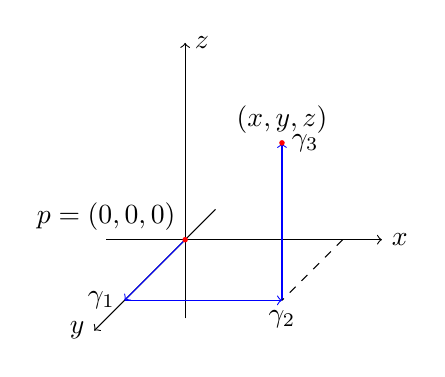
\begin{tikzpicture}
            \draw[->] (-1,0,0) -- (2.5,0,0) node[right] {$x$};
            \draw[->] (0,-1,0) -- (0,2.5,0) node[right] {$z$};
            \draw[->] (0,0,-1) -- (0,0,3) node[left] {$y$};
            %\node at (-1.2,0.5,0) {$p=(0,0,0)$};
            %\node at (2,2.5,2) {$(x,y,z)$};
            \draw[blue][->] (0,0,0) -- (0,0,2) node[black][left] {$\gamma_1$};
            \draw[blue][->] (0,0,2) -- (2,0,2) node[black][below] {$\gamma_2$};
            \draw[blue][->] (2,0,2) -- (2,2,2) node[black][right] {$\gamma_3$};
            \draw[dashed] (2,0,0) -- (2,0,2); % Linea discontinua
            \fill[red] (0,0,0) circle (1pt) node[black][above left] {$p=(0,0,0)$}; % Punto
            \fill[red] (2,2,2) circle (1pt) node[black][above] {$(x,y,z)$}; % Punto
        \end{tikzpicture}
    \end{center}

    Por lo tanto, $\vec{F}$ es conservativo.\\ De forma alternativa se podría haber
    visto que $\vec{F}$ es un campo conservativo, buscando una funcion $\varphi$
    tal que $\vec{F} = \nabla \varphi$, es decir:
    \begin{enumerate}
        \item $F_1 = \frac{\partial \varphi}{\partial x} = y \implies \varphi = xy + g(y,z)$
        \item $F_2 = \frac{\partial \varphi}{\partial y} = x + z\cos(yz) \implies \frac{\partial g}{\partial y} = z\cos(yz) \implies g = \sin(yz) + h(z)$
        \item $F_3 = \frac{\partial \varphi}{\partial z} = y\cos(yz) \implies \frac{\partial h}{\partial z} = y\cos(yz) \implies h = \frac{y}{z}\sin(yz) + c$
    \end{enumerate} $$\implies$$
    \begin{enumerate}
        \item $\varphi = \int \frac{d\varphi}{dx}dx = \int y dx = xy + H(y,z)$ constante con respecto a $x$
        \item $\frac{d\varphi}{dz} = \frac{dH}{dz} = y\cos(yz) \implies H = \int y\cos(yz)dz = \sin(yz) + G(y)$ constante con respecto a $z$
        \item $\frac{d\varphi}{dy} = \frac{d}{dy}(yx + \sin(yz) + G(y)) = x + z\cos(yz) + G'(y) = x + z\cos(yz) \implies G'(y) = 0 \implies G(y) = cte.$
    \end{enumerate}
}

\begin{proposición}
SEan $U \subset \mathbb{R}^n$ abierto y $\vec{F}: U \to \mathbb{R}^n$ campo conservativo de clase $C^1 \implies$ $$\frac{\partial F_i}{\partial x_j} = \frac{\partial F_j}{\partial x_i} \quad \forall i,j = 1, \ldots, n \text{ en } U$$
\end{proposición}
\begin{proof}
    Tomemos $\varphi: U \to \mathbb{R}$ tal que $\frac{\partial\varphi}{dx_i} = F_i \in C^1 \forall i = 1, \ldots, n$. Luego $\varphi$ es de clase $C^2$ y por el teorema de las derivadas cruzadas (Shcwartz) se tiene que:
    $$\frac{\partial}{\partial x_i}(F_j) = \frac{\partial^2 \varphi}{\partial x_i \partial x_j} = \frac{\partial^2 \varphi}{\partial x_j \partial x_i} = \frac{\partial}{\partial x_j}(F_i)$$
\end{proof}
\begin{corolario}
    Sean $U \subset \mathbb{R}^2$ abierto y $\vec{F} = (P, Q): U \to \mathbb{R}^2$ campo vectorial de clase $C^1$, entonces, si $\vec{F}$ es campo conservativo, se tiene que:
    $$\frac{\partial P}{\partial y} = \frac{\partial Q}{\partial x} \text{ en } U$$
    (Si $(P, Q) = \nabla \varphi \implies \frac{\partial P}{\partial y} = \frac{\partial^2 \varphi}{\partial y \partial x} = \frac{\partial^2 \varphi}{\partial x \partial y} = \frac{\partial Q}{\partial x}$ en U)
\end{corolario}
\begin{proof}
    $$\begin{cases}
            F_1 = P \\ F_2 = Q
        \end{cases}$$
\end{proof}
\begin{observación}
En general el recíproco no es cierto, depende de la forma del dominio ($U$).
\end{observación}
\begin{observación}
\underline{Terminología}:
\begin{itemize}
    \item Una forma diferencial de orden 1 en $U$ es una expresión de la forma $\omega =
              Pdx + Qdy$ con $P, Q$ de clase $C^1$ en $U$.
    \item $\omega$ es cerrada si $\frac{\partial P}{\partial y} = \frac{\partial Q}{\partial x}$ en $U$.
    \item $\omega$ es exacta si $\exists \varphi \in C^2(U) : \frac{\partial\varphi}{\partial x} = P, \frac{\partial Q}{\partial y} = Q \iff \nabla \varphi = (P, Q)$ en $U$.
\end{itemize}
Hemos visto que $\omega$ exacta $\implies$ $\omega$ cerrada.
\end{observación}


